\chapter{Introduction}


\section{Motivation and Background}


The growing global concern over climate change has significantly pressured industries to adopt sustainable practices. The maritime sector, responsible for approximately 30$\%$ of global CO\textsubscript{2} emmisions, has continuosly increased int emissions, as shown in Fig. 1.

\textcolor{blue}{https://theroundup.org/co2-greenhouse-gas-emission-statistics/}

\textcolor{blue}{https://www.container-xchange.com/blog/shipping-emissions/}

\begin{figure}[h!]
    \centering
    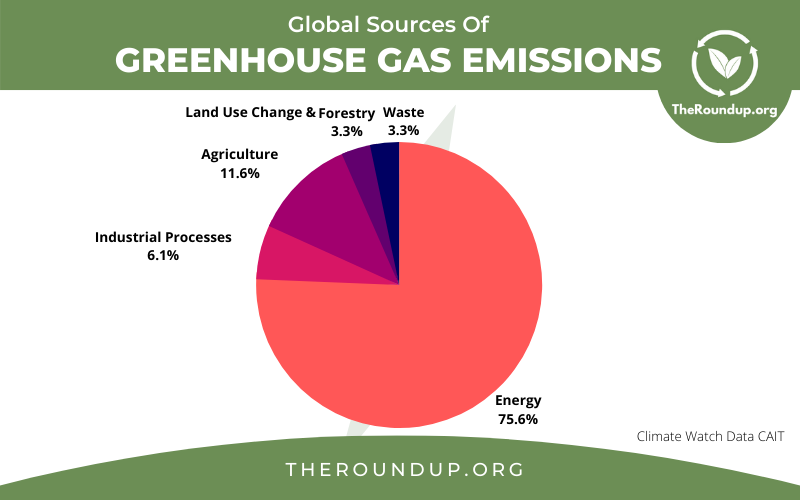
\includegraphics[width=0.9\textwidth]{images/chapter01/global_emss}
    \caption{Global sources of greenhouse gas emissions. Source: theroundup.org}
    \label{fig:global_emss}
\end{figure}

\begin{figure}[h!]

    \begin{subfigure}{0.5\textwidth}
    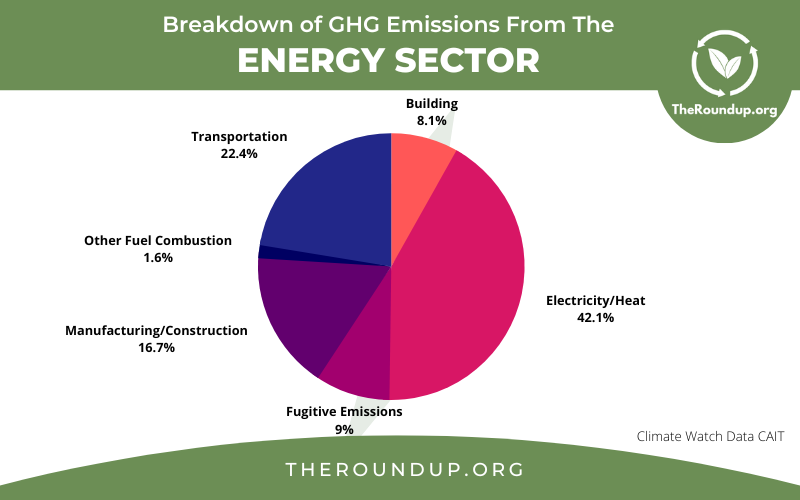
\includegraphics[width=1\textwidth]{images/chapter01/energy_emss.png}
    \caption{CO\textsubscript{2} emissions from the energy sector.}
    \label{fig:sub_energy}
    \end{subfigure}
    \begin{subfigure}{0.5\textwidth}
    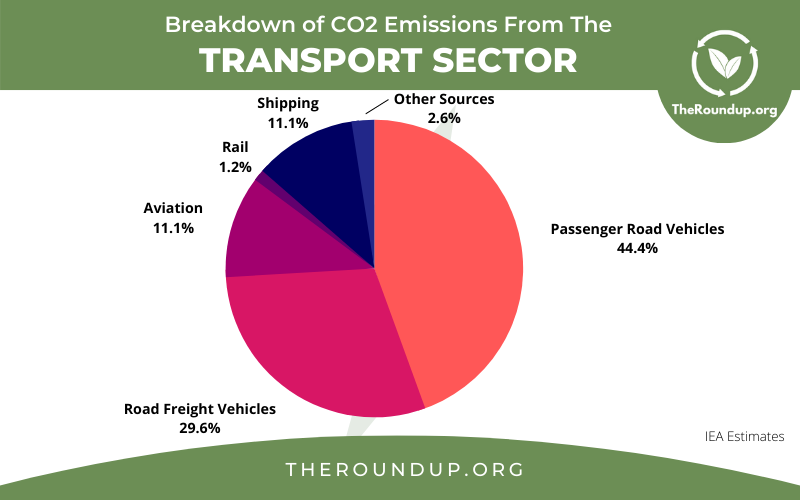
\includegraphics[width=1\textwidth]{images/chapter01/transport_emss.png}
    \caption{CO\textsubscript{2} emissions from the transport subsector.}
    \label{fig:sub_transport}
    \end{subfigure}
    
    \caption{Breakdown of CO\textsubscript{2} emissions from the energy sector and the transport subsector. Source: theroundup.org}
    \label{emss_2images}
\end{figure}

Addressing emission reduction is critical, as strict regulations on emissions and fuel efficiency aimed at mitigating the environmental impact of maritime activities are being implemented worldwide [2].

\begin{figure}[!h]
    \centering
    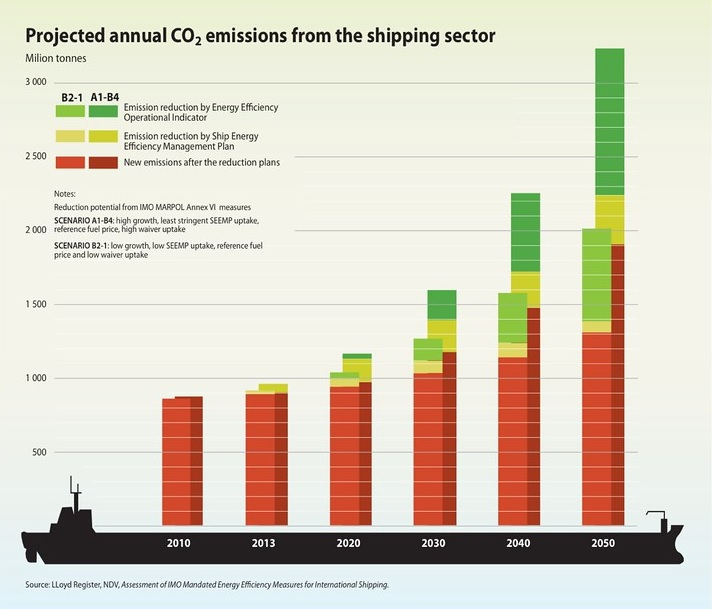
\includegraphics[width=0.85\textwidth]{images/chapter01/CO2_maritime_transport.jpg}
    \caption{IMO greenhouse gas emissions strategy. Source: Lloyd Register, NOV, Assestment of IMO Mandated Energy Efficiency Measures for International Shipping}
    \label{circuito_2}
\end{figure}

One promising approach is adopting electro-mobility technologies in maritime operations. In this context, electromobility can be implemented through various strategies [3], from hybrid propulsion systems to fully electric vessels [4]. Hybrid propulsion, in particular, combines the advantages of diesel engines with electric power systems, offering a flexible and efficient solution for reducing emissions without compromising performance [5]. The hybridization of propulsion systems relies on the separate or simultaneous use of different energy sources [1].

Several studies have examined hybrid propulsion systems. A marine hybrid propulsion system, focusing on vector control of the electric motor during different modes and verifying the control feasibility [6]. The optimization of hybrid propulsion system design for a tugboat has been explored, presenting a methodology that streamlines powertrain component sizing and control, minimizing costs for a specific operating profile [7]. A coordinated control strategy for a variable-speed hybrid tugboat have been presented to improve fuel economy. The proposed strategy, validated through simulations and a smallscale experimental testbed, showed reduced costs and lower CO2 emissions [8].

Among vessel types, tugboats—used for towing and maneuvering large ships—are among the highest emitters per unit of energy due to their highly variable load profiles [3]. Tugboats and ferries are ideal candidates for hybridization due to their operational profiles, which involve prolonged idling, low-speed maneuvering, and frequent speed changes that lead to inefficient fuel consumption [9].

This paper focuses on designing and sizing an energy storage system for a hybrid tugboat as a specific electro-mobility solution. Despite advancements in marine hybrid technologies, a standardized methodology for tugboat hybridization remains undefined [10]. The study presents a design methodology addressing parameters such as load profiles, power and energy demands, battery technology selection, and propulsion system optimization. Theoretical analysis is presented and simulation shows a emissions reduction while maintaining the robustness needed for towing and transit activities.

\section{Challenges and Research Opportunities}


\section{Thesis Objectives and Outline}




\cite{10735355},
\cite{10679076},
\cite{10472698},
\cite{10382632},
\cite{10269751},
\cite{10091779},
\cite{10136711},
\cite{10015728},
\cite{9937167},
\cite{9738734},
\cite{9913469},
\cite{9360490},
\cite{9340547},
\cite{9242285},
\cite{9184122},
\cite{9299429},
\cite{9046048},
\cite{8322257},
\cite{7945527},
\cite{8013775},
\cite{7956250},
\cite{7836306},
\cite{7604136},



